% REMEMBER: Write the thesis from the view of the reader. How would I like to READ the thesis?
% WHY -> WHAT -> HOW structure

% 6th, 7th grade

\chapter{Evaluation}%
\label{cha:evaluation}

TODO: Introduction

- In this chapter, the Whisker testing utility is evaluated

- 3 Parts
- TODO: explain RQs
    - 1. First it is shown that it is possible to run Whisker tests without interfering with the execution of the Scratch program
    - 2. The main part of the evaluation focuses on finding out how accurate Whisker's test results can be compared to manual assessment (normal + constraint tests)
    - 3. Then Whiskers random input is evaluated

- Chapter outline

\section{Experimental Setup}

\subsection{Testing Environment}

We used Whisker through its web GUI to execute test suites on several Scratch programs.
The software and hardware we used are listed in Figure~\ref{tab:evaluation_setup}.
All test executions were performed on the same machine.
Any programs running in the background were closed before running tests.
For two parts of the evaluation,
specifically to measure execution time and to measure coverage over time,
we used slightly modified versions of Whisker as well as its GUI.

\begin{table}[ht]
    \centering
    \scriptsize \tt
    \begin{tabular}{ll}
        \toprule
        Whisker     & Whisker 1.0 \\
        Scratch VM  & Scratch VM 0.2.0-prerelease.20181005173109 \\
        Web Browser & Chrome 70.0.3538.110 (64-Bit) \\
        JavaScript  & V8 7.0.276.40 \\
        OS          & Windows 8.1 Version 6.3 (Build 9600) \\
        CPU         & Intel Core i5 4670 (4 x  3.40 GHz) \\
        GPU         & Nvidia GeForce GTX 1080 \\
        RAM         & 8GB DDR3-1600 \\
        \bottomrule
    \end{tabular}
    \caption{Software and hardware used for evaluation}
    \label{tab:evaluation_setup}
\end{table}

\subsection{Projects Under Test}

This section will list the Scratch projects,
which we used to evaluate Whisker,
and explain, why these projects were chosen.

\subsubsection{(P1) Catching Game}

The first set of Scratch projects consists of 41 student implementations of a simple catching game.
The projects originate from a voluntary Scratch course for 6th and 7th grade students.
In this course, students were introduced to Scratch through several small exercises,
% familiarized themselves with Scratch
building up to the final and most complex exercise to develop the aforementioned catching game.
Students were given a project as a template to fill with their implementation.
\parspace

In this game, apples and bananas periodically fall from the top of the screen.
The player earns points by catching these fruits with a bowl at the bottom of the screen,
which is controlled with the left and right arrow keys.
The game ends when 30 seconds have passed or if an apple touches the ground.
A screenshot of the sample implementation of this program can be seen in Figure~\ref{fig:screenshot_of_the_sample_implementation}.
Additionally, a summary of the full program specification from the assignment may be found in Table~\ref{tab:project_specification}.
\mnote{TODO: assignment in the appendix?}
\parspace

\begin{figure}[ht]
    \centering
    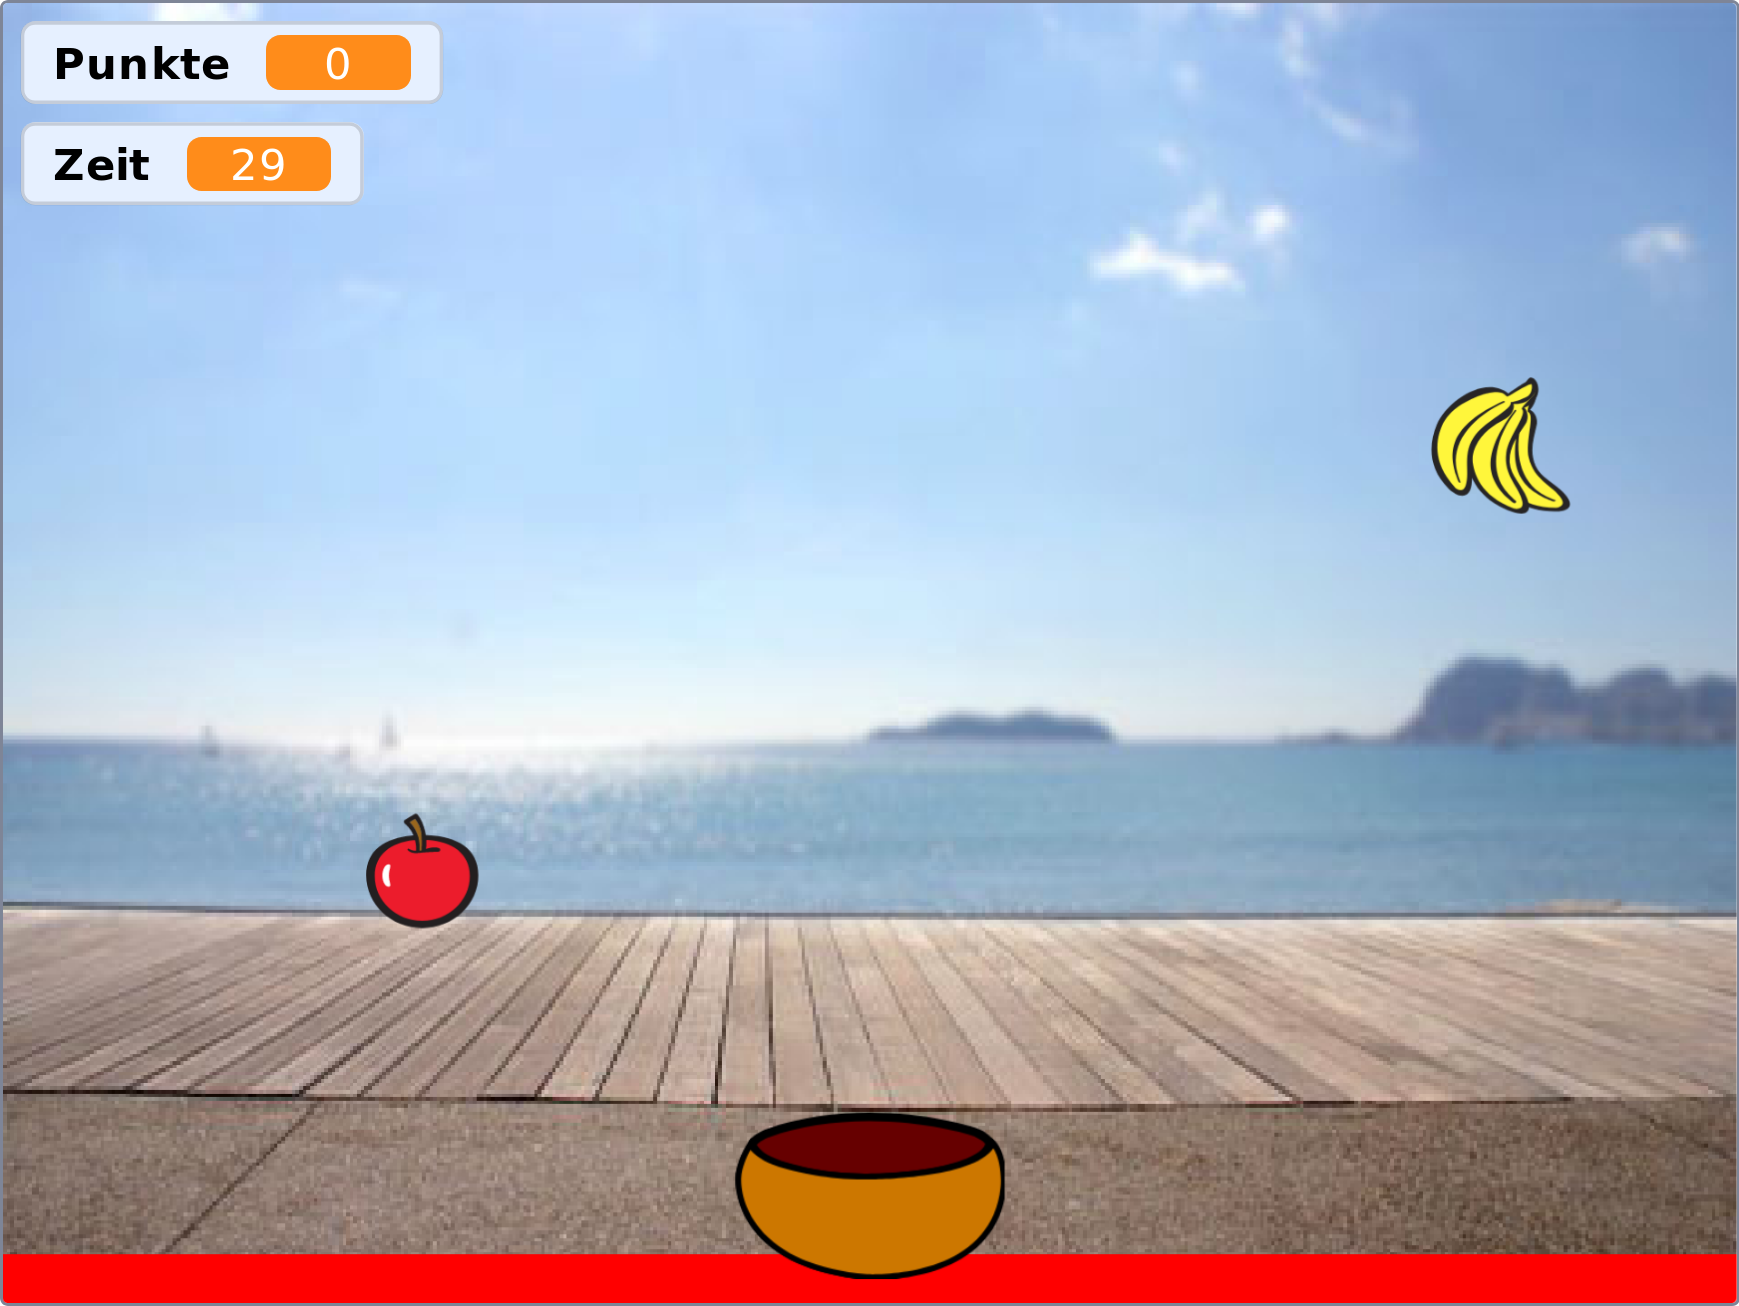
\includegraphics[width=0.35\textwidth]{scratch-stage}
    \caption{Screenshot of the sample implementation}
    \label{fig:screenshot_of_the_sample_implementation}
\end{figure}

We will execute different test suites on these programs to analyze the quality of test results.
The projects are suitable for this task because of two reasons.
The task description specifies the program well, which enables us to write automated tests according to the specification.
Secondly, the student solutions are of varying degrees of quality,
which is desirable, so automated tests produce a range of different outcomes.
% Some of the projects implement the game almost perfectly,
% while many contain common errors, and some don't work correctly at all.
However, testing these projects has also revealed some challenges.
For one thing, these projects were never meant to be subject to automated testing.
Therefore, some details, mainly the usage of clones,
are not part of the task specification, which complicates testing,
since tests have to consider multiple options.
Additionally, the game over state, that the program enters,
when an apple touches the ground, also makes automated testing more difficult.
\parspace

Since the students didn't write the programs with automated testing in mind,
some of the projects were unusable for our evaluation, so we excluded them from the statistics.
Table~\ref{tab:excluded_projects} shows the excluded projects together with the reasons for excluding them.
The projects are named K6\_S01 through K6\_S33 for 6th grade student solutions
and K7\_S02 through K7\_S27 for 7th grade student solutions respectively (with many numbers being skipped).
Most of the excluded projects were found by analyzing the test reports and the coverage of our test suite,
while two of them were detected manually from a discrepancy between our test results and the manual scoring,
which we will compare our results to later.

% === Excluded Projects
% - Some of the projects were excluded from the evaluation
% - Because they where problematic to automated testing in some way
%     - Tests select sprites and variables by name, and some projects changed the names of sprites and variables
%         - Detected by searching the test reports: ''grep''
%     - Some projects used a different mechanism than the green flag to start their program
%         - Since this is not specified, tests can not start the program
%         - Detected by zero statement coverage
%     - Some Projects didn't work properly because of missing initialization
%         - Go game over on startup
%         - One project work if green flag is pressed multiple times
%         - One project only worked if the sprites were manually dragged to a different position

\begin{table}
    \centering
    \scriptsize
    \begin{tabular}{ll}
        \toprule
        Project & Reason                                                                          \\
        \midrule
        \multicolumn{2}{l}{\textbf{Detected through the test report}}                             \\
        K6\_S12 & Deleted variable from template: ''Zeit''                                        \\
        K6\_S17 & Renamed variable from template: ''Punkte'' to ''Bunkte''                        \\
        K7\_S24 & Deleted variable from template: ''Zeit''                                        \\
        K7\_S27 & Renamed sprite from template: ''Bowl'' to ''Figur2''                            \\[\medskipamount]

        \multicolumn{2}{l}{\textbf{Detected through zero statement coverage}}                     \\
        K6\_S01 & Starts on up arrow key press instead of green flag                              \\
        K6\_S06 & Wrong scratch project file (scored 30 points in manual rating but has no code)  \\
        K6\_S14 & Starts on space key press instead of green flag                                 \\[\medskipamount]

        \multicolumn{2}{l}{\textbf{Detected manually}}                                            \\
        K6\_S20 & Green flag has to be pressed twice to make it work properly                     \\
        K7\_S18 & Sprites have to be repositioned manually in the editor to make it work properly \\
        \bottomrule
    \end{tabular}
    \caption{Excluded projects together with the reason to exclude them}
    \label{tab:excluded_projects}
\end{table}

\subsubsection{(P2) Code Club Projects}

The second set of Scratch projects consists of sample solutions to 24 of Code Club's~\cite{codeclub} Scratch exercises.
Code Club offers free coding projects and step by step guide for programming beginners.
For each project, a sample solution is provided by a volunteer.
\parspace

\mnote{Add a table which lists the projects?}
We use these projects to evaluate Whisker's automated test input generation by measuring its achieved coverage.
The projects work well for this task since they implement a variety of different programs with different input methods.
We chose the sample solutions of the exercises since measuring coverage on working implementation will yield better results.
Broken implementations may be more likely to have unreachable code,
because code might depend on a feature, that is not implemented correctly.

\subsection{Test Suites}

The set of catching game projects (P1) will be tested with three different test suites.
Table~\ref{tab:project_specification} lists which part of the project specification is covered by each test suite.

\begin{table}
    \centering
    \scriptsize
    \begin{tabular}{rlccc}
        \toprule
        \texttt{\#} & Specification                                                                & T1     & T2, T3                    & T4                        \\
        \midrule
           & \textbf{Initialization} \\
         1 & Timer starts at 30 seconds                                                            & \cmark & \xmark                    & \xmark                    \\
         2 & Bowl starts at $X = 0$ / $Y = -145$                                                   & \cmark & \xmark                    & \xmark                    \\
         3 & Fruits have a size of 50\%                                                            & \cmark & \cmark                    & \cmark                    \\[\medskipamount]
           & \textbf{Bowl Movement} \\
         4 & Bowl moves left/right when corresponding arrow key is pressed                         & \cmark & \cmark                    & \cmark                    \\
         5 & Bowl can only move horizontally with a speed of 10                                    & \cmark & \cmark                    & \cmark                    \\[\medskipamount]
           & \textbf{Fruit Falling} \\
         6 & Apples fall down                                                                      & \cmark & \textasteriskcentered$^1$ & \textasteriskcentered$^1$ \\
         7 & Apples fall in a straight line with a speed of -5                                     & \cmark & \cmark                    & \cmark                    \\
         8 & Bananas fall down                                                                     & \cmark & \textasteriskcentered$^2$ & \textasteriskcentered$^2$ \\
         9 & Bananas fall in a straight line with a speed of -7                                    & \cmark & \cmark                    & \cmark                    \\[\medskipamount]
           & \textbf{Fruit Spawn} \\
        10 & Apples spawn again at the top of the screen after touching the bowl                   & \cmark & \textasteriskcentered$^3$ & \xmark                    \\
        11 & Apples spawn at random $X$ position                                                   & \cmark & \cmark                    & \xmark                    \\
        12 & Apples spawn at $Y = 170$                                                             & \cmark & \cmark                    & \xmark                    \\
        13 & Bananas spawn again at the top of the screen after touching the bowl                  & \cmark & \textasteriskcentered$^4$ & \xmark                    \\
        14 & Bananas spawn at random $X$ position                                                  & \cmark & \cmark                    & \xmark                    \\
        15 & Bananas spawn at $Y = 170$                                                            & \cmark & \cmark                    & \xmark                    \\
        16 & Only one apple must fall down at a time                                               & \cmark & \cmark                    & \xmark                    \\
        17 & Only one banana must fall down at a time                                              & \cmark & \cmark                    & \xmark                    \\
        18 & Banana must wait for a second before falling down in the beginning                    & \cmark & \xmark                    & \xmark                    \\
        19 & Banana must wait for a second before falling down after displaying the ''-8'' message & \cmark & \xmark                    & \xmark                    \\[\medskipamount]
           & \textbf{Fruit Interaction} \\
        20 & Apple gives 5 points when it touches the bowl                                         & \cmark & \cmark                    & \cmark                    \\
        21 & Game over when the apple touches the ground                                           & \cmark & \textasteriskcentered$^5$ & \cmark                    \\
        22 & Apple displays ''Game Over!'' message when it touches the ground                      & \cmark & \textasteriskcentered$^5$ & \cmark                    \\
        23 & Banana gives 8 points when it touches the bowl                                        & \cmark & \cmark                    & \cmark                    \\
        24 & Banana subtracts 8 points when it touches the ground                                  & \cmark & \cmark                    & \cmark                    \\
        25 & Banana displays ''-8'' message when it touches the ground                             & \cmark & \cmark                    & \cmark                    \\[\medskipamount]
           & \textbf{Timer} \\
        26 & Timer ticks down                                                                      & \cmark & \cmark                    & \cmark                    \\
        27 & Game stops when timer reaches 0                                                       & \cmark & \cmark                    & \xmark                    \\
        28 & Bowl must display ''Ende!'' message when timer reaches 0                              & \cmark & \cmark                    & \xmark                    \\
        \bottomrule \\
        \textasteriskcentered$^1$ & Not covered directly, because indirectly covered by (7) \\
        \textasteriskcentered$^2$ & Not covered directly, because indirectly covered by (9) \\
        \textasteriskcentered$^3$ & Not covered directly, because indirectly covered by (11), (12) \\
        \textasteriskcentered$^4$ & Not covered directly, because indirectly covered by (14), (15) \\
        \textasteriskcentered$^5$ & Covered, but game over through apple not expected to happen \\
    \end{tabular}

    \caption{Project specifications and their coverage by the test suites}
    \label{tab:project_specification}
\end{table}

\subsubsection{(T1) Normal Test Suite}

This test suite follows an ordinary testing approach.
Each test case runs the program once in order to check one part of the specification.
Tests simulate inputs deliberately and mostly perform assertions between runs of the program.
Listing~\ref{lst:example_test_case_normal} shows a shortened example of a simple test case from this test suite.
% which tests the user interaction with the bowl sprite.
The test suite encompasses 28 test cases, which correspond to the specification in Table~\ref{tab:project_specification}.
\parspace

\begin{listing}[ht]
    \centering
    \begin{minipage}{.70\textwidth}
        \begin{minted}[autogobble, breaklines, linenos, fontsize=\scriptsize, framesep=2mm, frame=lines]{javascript}
            const testMoveBowl = async function (t, testDetails = false) {
                const {bowl} = getSpritesAndVariables(t, ['bowl']);
                let bowlX;

                /* Give the program some time to initialize. */
                await t.runForTime(250);

                /* Test movement when no key is pressed. */
                bowlX = bowl.x;
                await t.runForTime(250);
                t.assert.equal(bowl.x, bowlX,
                    'Bowl must not move when no key is pressed.');

                /* Test movement when left arrow key is pressed. */
                t.inputImmediate({
                    device: 'keyboard',
                    key: 'left arrow',
                    isDown: true,
                    duration: 50
                });
                bowlX = bowl.x;
                await t.runForTime(250);
                t.assert.less(bowl.x, bowlX,
                    'Bowl must move to the left when left arrow key is pressed.');

                /* Test movement when right arrow key is pressed. */
                ...
            };
        \end{minted}
    \end{minipage}

    \caption{Shortened example test case from test suite T1}
    \label{lst:example_test_case_normal}
\end{listing}

For many tests, the catching game has to be played without letting an apple touch the ground for a period of time.
In order to accomplish this we implemented a helper function,
which takes the x coordinates of the apple and bowl sprites and
simulates arrow key presses to move the bowl towards the apple's position.
This function, as well as a usage example, are shown in Listing~\ref{lst:simulating_catching_game}.

\begin{listing}[ht]
    \centering
    \begin{minipage}{.85\textwidth}
        \begin{minted}[autogobble, breaklines, linenos, fontsize=\scriptsize, framesep=2mm, frame=lines]{javascript}
            const followSprite = function (t, bowlX, spriteX) {
                /* Stop if the bowl is near enough. */
                if (Math.abs(bowlX - spriteX) <= 10) {
                    t.inputImmediate({device: 'keyboard', key: 'left arrow',  isDown: false});
                    t.inputImmediate({device: 'keyboard', key: 'right arrow', isDown: false});

                } else if (bowlX > spriteX) {
                    t.inputImmediate({device: 'keyboard', key: 'right arrow', isDown: false});
                    t.inputImmediate({device: 'keyboard', key: 'left arrow',  isDown: true});

                    /* Trick "when key pressed" hats to fire by letting go of the key and immediately pressing it again. */
                    t.inputImmediate({device: 'keyboard', key: 'left arrow',  isDown: false});
                    t.inputImmediate({device: 'keyboard', key: 'left arrow',  isDown: true});

                } else if (bowlX < spriteX) {
                    t.inputImmediate({device: 'keyboard', key: 'left arrow',  isDown: false});
                    t.inputImmediate({device: 'keyboard', key: 'right arrow', isDown: true});

                    /* Trick "when key pressed" hats to fire by letting go of the key and immediately pressing it again. */
                    t.inputImmediate({device: 'keyboard', key: 'right arrow', isDown: false});
                    t.inputImmediate({device: 'keyboard', key: 'right arrow', isDown: true});
                }
            };

            const testSomething = function (t) {
                ...
                /* Catch apples with the bowl during runs. */
                t.addCallback(() => {
                    apple = getNewestClone(apple);
                    followSprite(t, bowl.x, apple.x);
                });
                ...
            };
        \end{minted}
    \end{minipage}

    \caption{Simulating arrow key presses to play the catching game}
    \label{lst:simulating_catching_game}
\end{listing}

\subsubsection{(T2) Input-Independent / Constraint-Only Test Suite}

This test suite implements the input-independent testing approach from Chapter~\ref{cha:using_constraints_to_enable_flexible_test_inputs}.
With this test suite, we tried to test the program with only one execution in total.
Therefore, this test suite only has one test case, which registers 20 constraints to check various parts of the specification
(again corresponding to Table~\ref{tab:project_specification}).
\parspace

This test case deliberately simulates inputs with the goal of winning the game.
We use the same helper method as test suite T1 to simulate key presses depending on the bowl's and the apple's position.
Because of this, the bowl should always catch the apple in working implementations,
and the program should never go game over because of an apple touching the ground.
Nevertheless, we register constraints, which check the game over state in case an apple does reach the ground in a buggy implementation.

\subsubsection{(T3) Random Input Tests}

\mnote{TODO: table with number of tests and LOC of each test suite}
Test suite T3 is exactly identical to test suite T2,
but uses Whisker's automated test input generation instead of deliberately simulating inputs.
Listing~\ref{lst:automated_input_random_tests} shows the exact code snippet, which simulates input for the test case.
\parspace

\begin{listing}[ht]
    \centering
    \begin{minipage}{.45\textwidth}
        \begin{minted}[autogobble, breaklines, linenos, fontsize=\scriptsize, framesep=2mm, frame=lines]{javascript}
            t.setRandomInputInterval(150);
            t.detectRandomInputs({duration: [50, 100]});
        \end{minted}
    \end{minipage}
    \caption{Automated input generation for random test suites}
    \label{lst:automated_input_random_tests}
\end{listing}

\subsubsection{(T4) Lite Random Input Tests}

Since performing inputs randomly will likely result in the falling apple touching the ground,
we added T4 as a variant of T3.
T4 works on the assumption, that the first apple will touch the ground and cause a game over.
Therefore, T4 doesn't test anything, which requires the test to successfully catch the apple with the bowl.
It only registers the 12 of T3's 20 constraints, that are relevant for the first few seconds of the program execution.
Otherwise, T4 is identical to T3.

\section{RQ1: Interference with the Program Under Test}

Since the tests execute code between steps in a single threaded environment,
they could, in theory, interfere with the program by slowing down the step cycle.
This can make the program behave differently, because Scratch programs use absolute timings (TODO figure).

~\\~\\
\textbf{RQ1.} typical tests don't interfere with the execution of typical Scratch programs
$\rightarrow$ measure how long Scratch takes for a step (WORK\_TIME AND time to render)
$\rightarrow$ measure how long each operation in the Whisker step procedure takes (e.g. callbacks, sprites, constraints)
$\rightarrow$ Explain how the times are measured

TODO: explain why testing procedure might interfere with Scratch programs (absolute timings)
TODO: timing diagram and table of timings for real tests
TODO: example code for tests that interfere and their test data

~\\~\\
\paragraph{Null hypothesis ($H_0$)}
Additional computations for testing are to slow to be executed while the program is running and stretch out the average time a step takes.
\paragraph{Alternative hypothesis ($H_1$)}
Additional computations for testing can be fast enough to not affect the average step time.

\section{RQ2: Accuracy of Test Results}
% \subsection{Evaluation Method}
% \subsection{Data Selection}
% \subsection{Threats to Validity}

\textbf{RQ2.}
- Automatic testing can facilitate grading of Scratch assignments
    (1) test results (normal tests and constraint tests) match the results of manual evaluation
    (3) test results (normal tests and constraint tests) are consistent enough to be used for grading
        $\rightarrow$ Plot difference number of test passes per project
        $\rightarrow$ Check average difference

- Manual analysis is used as ground truth

TODO: explain why accuracy is evaluated in this way
    - attention to automated grading
TODO: discuss scatter and bar plots

~\\~\\
=== (1)
\paragraph{Null hypothesis ($H_0$)}
Test results have no strong relation to the scores that were given to the projects manually.
\paragraph{Alternative hypothesis ($H_1$)}
The results of automated tests closely match the results of manual scoring.

~\\~\\
=== (2)
\paragraph{Null hypothesis ($H_0$)}
Automated test results show very different results each run and are thus not accurate enough to use them for grading.
\paragraph{Alternative hypothesis ($H_1$)}
Test results are consistent enough over multiple runs to provide accurate information for grading.

\section{RQ3: Testing with Random Inputs}

\mnote{Add the random input ''test''}

\textbf{RQ3.}
- The testing process can be done entirely in the background independent of testing scenarios (?)
    $\rightarrow$ Random input can be used for the test
    $\rightarrow$ The test can involve the user using the program like they normally would

% - Constraint Tests
%     - Different approach: One test executes the program only once and checks defined constraints in the background, see Section \ref{sec:constraint_only_tests}
%     - Deliberately control the bowl to win the game
%     - faster, but can be less accurate (show difference of average runtime)
%     - not everything in this project can be tested in a single run
%     - Better for quickly checking the program
%     - Example of a constraint test (or put it somewhere else?)
%     - Can be used with different sources of input (manual / simulated / random)
%     - Instead of passing tests, passing constraints are measured
%     - Tests with wrong sprite names are completely excluded in the evaluation

- Automatic test input generation
- Same constraints as the constraint tests vs. only constraints that can hold in the first few seconds every time
    - Random input instead of deliberately controlling the bowl
    - Useful to test the stability of the program (like Android Monkey \cite{androidmonkey})
    - The catching game is not well suited for this approach since random input will quickly result in a game over

TODO: discuss test results
TODO: discuss coverage results


\section{Threats to validity}
- Students often deliberately changed their programs from the specification (e.g. different fall speeds)
    - Tests were adjusted to allow a little more than the specification (e.g. different message)

- For each tests suite, many / all projects were executed in a row
    - Could have a performance impact (?), but Scratch doesn't need a lot of resources
    - If anything, it could have a negative impact on the results, but results are very positive

- Tests could interfere with the program under test (see prev. section)
    - But Scratch programs don't usually do calculations without moving any sprite
    - Most time related functionality is based on absolute time, slow-down would not affect it

- Browser JavaScript could be problematic

% \begin{figure}
%     \centering
%     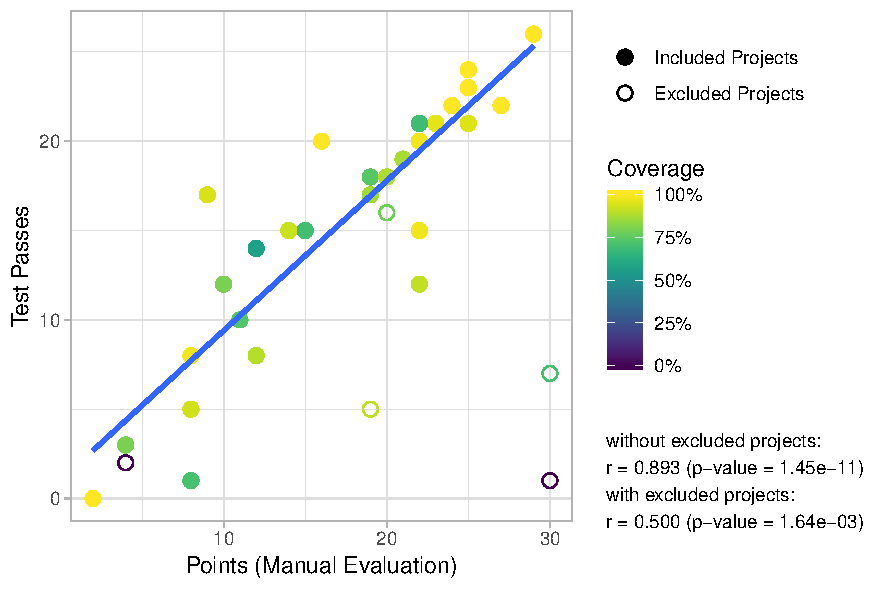
\includegraphics[width=.65\textwidth]{scatter-normal-1}
%     \caption{Results of the normal test suite (1)}
%     \label{fig:scatter_normal_1}
% \end{figure}
%
% \begin{figure}
%     \centering
%     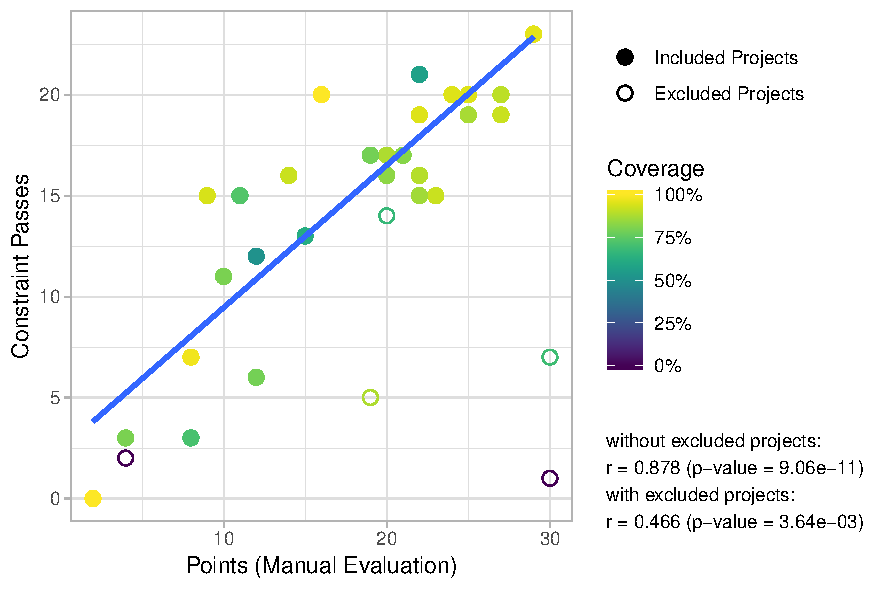
\includegraphics[width=.65\textwidth]{scatter-constraint-1}
%     \caption{Results of the constraint test suite (2) \\ with deliberately simulated input}
%     \label{fig:scatter_constraint_1}
% \end{figure}
